\subsection{Two Pods Different Node}
\subsubsection{Two Pods Different Node CPU Utilization}
\begin{itemize}
    \item In the two-pod-diff-node configuration, CPU utilization may vary depending on the distribution of workload across the two pods located on different nodes.
    \item Since each pod is on a different node, the workload is distributed evenly, potentially balancing the overall CPU usage across nodes.
    \item CPU utilization may vary as each pod handles its respective requests, but overall utilization may stabilize over time.
\end{itemize}

\noindent Below is the graph that illustrates the CPU utilization for the two-pod-diff-node configuration:

\begin{figure}[h]
    \begin{minipage}[t]{0.5\textwidth}
        \centering
        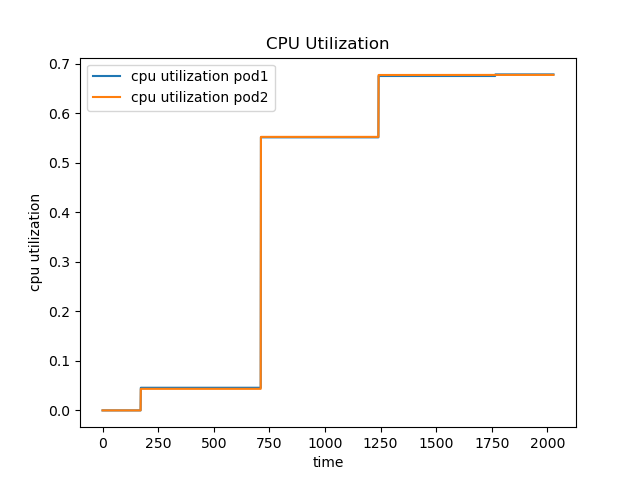
\includegraphics[width=0.9\textwidth]{../sample_results/loop/two-pod-diff-node/cpu-utilization-two-pod-diff-node.png}
        \caption{Loop}
    \end{minipage}
    \hfill
    \begin{minipage}[t]{0.5\textwidth}
        \centering
        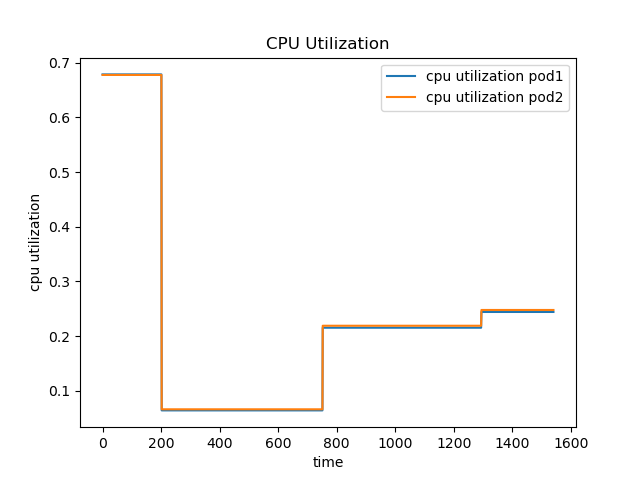
\includegraphics[width=0.9\textwidth]{../sample_results/lorem/two-pod-diff-node/cpu-utilization-two-pod-diff-node.png}
        \caption{Lorem}
    \end{minipage}
\end{figure}

\newpage
\subsubsection{Two Pods Different Node Response Time Observations}
\begin{itemize}
    \item Response times in the two-pod-diff-node configuration may be consistent due to the even distribution of workload across the two pods on different nodes.
    \item The setup allows each pod to handle requests independently, possibly balancing the load and resulting in more consistent response times.
    \item Under peak demand, response times may increase if either pod becomes overwhelmed, but overall, the configuration tends to provide more consistent response times.
\end{itemize}

\noindent Below are the response time graphs for the two-pod-diff-node configuration:

\begin{figure}[h]
    \begin{minipage}[t]{0.5\textwidth}
        \centering
        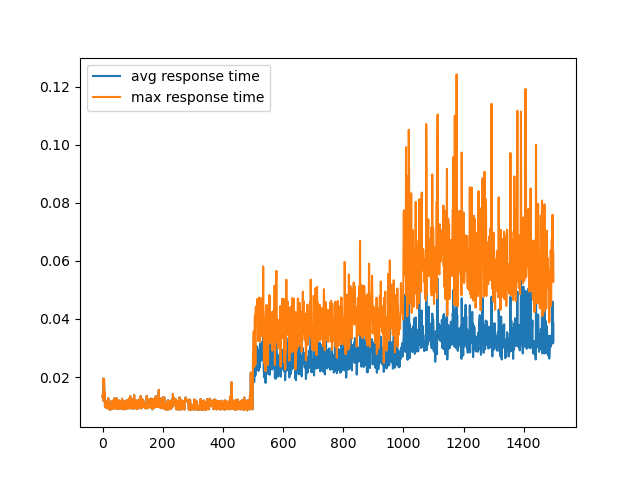
\includegraphics[width=0.9\textwidth]{../sample_results/loop/two-pod-diff-node/response-time-two-pod-diff-node-two-pod-diff-node.png}
        \caption{Loop}
    \end{minipage}
    \hfill
    \begin{minipage}[t]{0.5\textwidth}
        \centering
        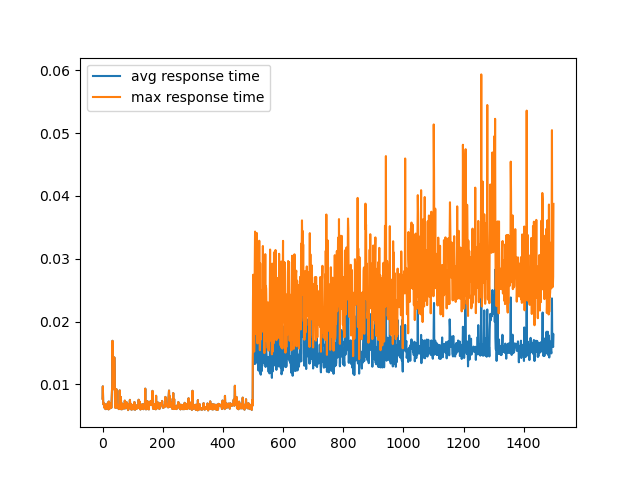
\includegraphics[width=0.9\textwidth]{../sample_results/lorem/two-pod-diff-node/response-time-two-pod-diff-node-two-pod-diff-node.png}
        \caption{Lorem}
    \end{minipage}
\end{figure}

\newpage
\subsubsection{Two Pods Different Node Memory Utilization}
\begin{figure}[h]
    \begin{minipage}[t]{0.5\textwidth}
        \centering
        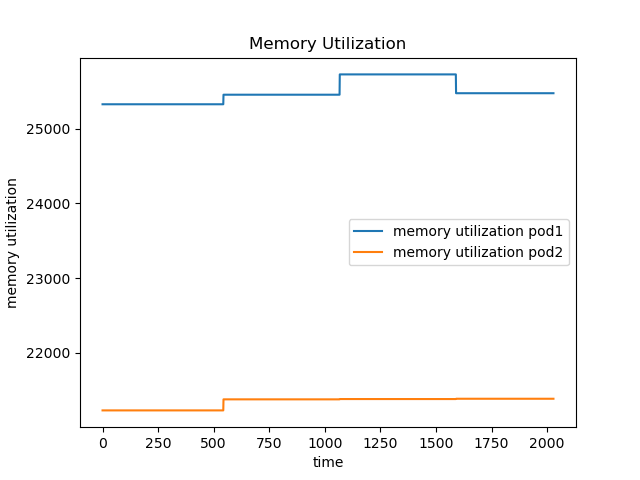
\includegraphics[width=0.9\textwidth]{../sample_results/loop/two-pod-diff-node/mem-utilization-two-pod-diff-node.png}
        \caption{Loop}
    \end{minipage}
    \hfill
    \begin{minipage}[t]{0.5\textwidth}
        \centering
        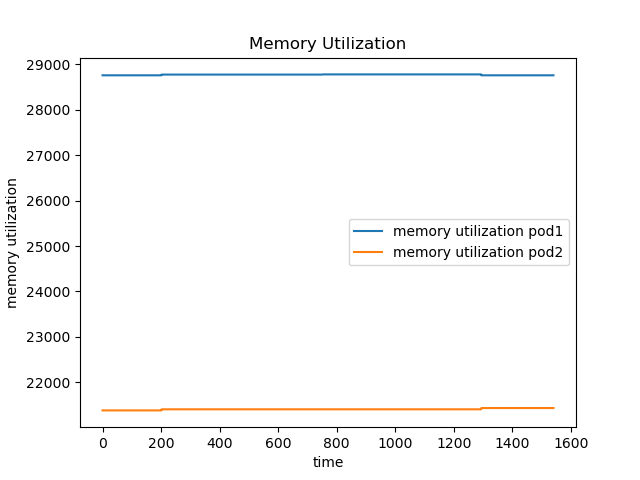
\includegraphics[width=0.9\textwidth]{../sample_results/lorem/two-pod-diff-node/mem-utilization-two-pod-diff-node.png}
        \caption{Lorem}
    \end{minipage}
\end{figure}

\begin{itemize}
    \item Memory utilization in the two-pod-diff-node configuration can vary depending on the memory requirements of each pod on different nodes.
    \item Since the pods are on separate nodes, memory usage is isolated per pod, potentially leading to efficient usage of resources.
    \item As workloads stabilize, memory utilization tends to balance out as each pod manages its own resources independently.
\end{itemize}

